\chapter{State of the Art}
\label{chap:soa}

This chapter will introduce the main concepts and tools that will be used during the development 
of the project. The \autoref{sec:abr} will explain the different methods of content distribution 
over \textit{HTTP} and different types and implementations of adaptive streaming.
The \autoref{sec:dash} will make a introduction to 
the \textit{DASH} standard, different types of adaptation algorithms and \textit{QoE} and 
\textit{QoS} metrics. The \autoref{sec:4g} will describe basic architecture and fundamentals
of 4G LTE, such as the radio interface, propagation loss model, fading model, antenna model, etc.

\section{ABR Video Streaming}
\label{sec:abr}

There are three ways of media delivery over \textit{HTTP}. The first method is by
\textbf{file download}, the media file is downloaded in its entirety in a local hard disk and 
then it can be played. The second method is called \textbf{progressive download}, this method
is similar to the file download, but instead the download starts from the beginning and the 
media starts playing once enough data are playable. 
However, these two methods have disadvantages like waste of bandwidth or
\textit{DRM} issues and also requiring a reliable transmission. The last method is called
\textbf{streaming}, contrary to the former two, the file itseft is not stored locally, 
smaller chunks of video are sent from the server and the client needs a data buffer to store 
the data that is being downloaded. The client plays the multimedia content from the 
buffer, and when the session is closed the data are deleted.

Streaming media also comes with some challenges. There are a lot of network variability
and a big heterogeneity in video capable devices. Therefore, to overcome these shortcomings,
\textit{Adaptive bitrate streaming (ABR)} was created.

The basic idea of \textit{Adaptive bitrate streaming} is to adapt the media content
for the user by monitoring different parameters like estimated bandwidth, buffer level or
\textit{CPU load}, see \autoref{fig:abrtime}. There are many propietary adaptive streaming solutions:

\begin{itemize}[topsep=0.5pt]
  \setlength\itemsep{0.5pt}
  \item \textbf{\textit{Apple HTTP Live Streaming (HLS)}}: \textit{HTTP Live Streaming HLS}
  is an implementation of an \textit{ABR} protocol over \textit{HTTP} developed by Apple \cite{hls1}
  as part of the QuickTime software and the mobile operating system \textit{iOS}. \textit{HLS} 
  supports live streaming and video on demand. \textit{HLS} is proposed in 2009 as a standard to
  the \textit{IETF} \cite{hls2}.
  \item \textbf{\textit{Microsoft Smooth Streaming (MSS)}}: \textit{Smooth Streaming} is part
  of \textit{Internet Information Services (IIS) Media Services} for delivering media over
  \textit{HTTP} \cite{mss1}. Their \textit{MSS} technology was used for several
  sports events such a the Beijing Summer Olympic Games in 2008 and the 2010 Winter Olymplics
  in Vancouver \cite{mss2}.
  \item \textbf{\textit{Adobe HTTP Dynamic Streaming (HDS)}}: \textit{HTTP Dynamic Streaming}
  is the implementation of adaptive streaming by Adobe. \textit{HDS} enables high-quality, network
  efficient HTTP streaming for media delivery that is tightly integrated with Adobe software \cite{hds1}. The
  solution is based in using \textit{Open Source Media Framework (OSMF)} and Adobe Flash Player.
\end{itemize}

\begin{figure}[h]
  \centering
  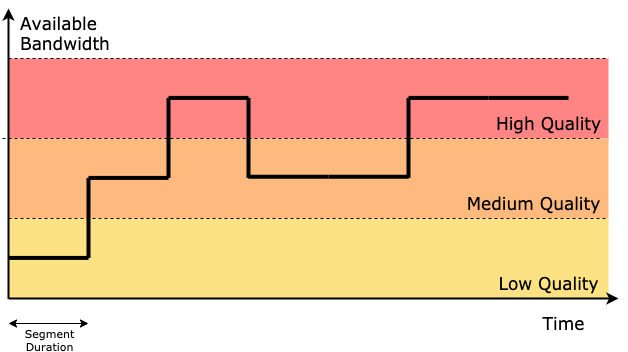
\includegraphics[width=0.7\textwidth]{img/abrtime.png}
  \caption{Evolution of segment quality with time}
  \label{fig:abrtime}

\end{figure}

But there was no official standarization for adaptive video delivery over HTTP. For that reason,
a new international stadard called \textit{MPEG-DASH} was developed and published.

\section{Dynamic Adaptive Streaming over HTTP}
\label{sec:dash}

\textit{DASH} was published in April 2012. 
The most recent revision of the standarization was released in 2019 as 
\textit{MPEG-DASH ISO/IEC 23009-1:2019} \cite{ISO23009}. 
 \textit{Moving Picture Experts Group} from \textit{ISO/IEC} and the \textit{3GPP} collaborated on
the \textit{DASH} standard. The \textit{3\textsuperscript{rd} Generation Partnership Project} defined the use of
\textit{DASH} as the standard of digital media delivery in mobile networks (4G \textit{LTE}, 5G) in \cite{3gpp1}.

The objective of \textit{DASH} was to create a unique standard that unifies the propietary solutions
from Microsoft, Apple and Adobe. Also, it will offer the interoperability and the convergence needed for 
the expansion of large-scale video streaming solutions. Also, the \textit{DASH Industry Forum (DASH-IF)} was created to promote and help the expansion of
\textit{DASH}. Microsoft, Apple, Netflix, Qualcomm, Ericsson and Samsung are some of the companies
members of the \textit{DASH-IF}.

One of the biggest advantages of \textit{DASH} is the use of \textit{HTTP} protocol.
The use of \textit{HTTP} means that reusing existing internet infrastructure and
media content distribution tecniques using \textit{CDN (Content Delivery Networks)} can be done.
Another convenience of using \textit{DASH} is, problems
with passing through firewalls and the \textit{Network Address Translation (NAT)}
are avoided.

All the control of the media content delivery is located in the \textit{DASH} client side. The
standard does not define any web delivery mechanism nor the bitrate adaptation algorithm. What \textit{DASH}
does define in \cite{ISO23009} is:

\begin{itemize}
  \item \textit{\textbf{The Media Presentation Description (MPD) File Format}}: The \textit{MPD} file
  uses the \textit{eXtensible Markup Language (XML)} and
  contains the specifications of the media content and the \textit{URL} of the segments
  in the \textit{HTTP} video servers.
  \item \textbf{Segment format}: \textit{DASH} defines the characteristics of the necessary
  codifications and the way that the media content is divided in small fragments called 
  \textit{segments}.
\end{itemize}


\begin{figure}[h]
  \centering
  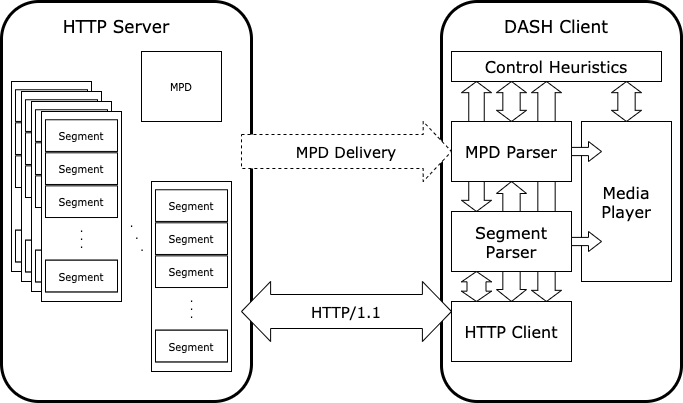
\includegraphics[width=0.7\textwidth]{img/dasharch.png}
  \caption{DASH client-server architecture. Source: MPEG \cite{ios1}}
  \label{fig:dasharch}
\end{figure}

The \autoref{fig:dasharch} presents a simple \textit{DASH} architecture. The video and audio
contents are processed and stored on an \textit{HTTP} server. To access the content, the client
sends \textit{HTTP} requests to the server. But first, the client needs to download the 
\textit{MPD} file, normally through \textit{HTTP}. The client then does the
parsing of the \textit{MPD}, extract information such as the duration of a segment, 
the available representations, media types or 
resolutions. Finally, the \textit{DASH} client chooses the adequate quality and starts the 
streaming of the content using \textit{HTTP GET} request to fetch the segments.

The \textit{DASH} client stores the segments in a buffer and consumes the content. The adaptation
algorithm selects the most appropiate representation, for example, basing on bandwidth estimations,
to avoid problems like buffer underflow and maintain at 
least a set number of segments in the buffer.

\subsection{MPD}
\label{sec:mpd}
The \textit{MPD} file is an \textit{XML} document that describes the characteristics
of the different media components that composes the media content (e.g. video, audio, subtitles).

The structure of the \textit{MPD} is hierarchical as illustrated in \autoref{fig:mpd}. The media content is divided in a sequence of
\textbf{periods}, where each period has a starting time and a duration. During a period, the set of characteristics
of the media content, like the bitrates, languages or codecs, do not change.

\begin{figure}[h]
  \centering
  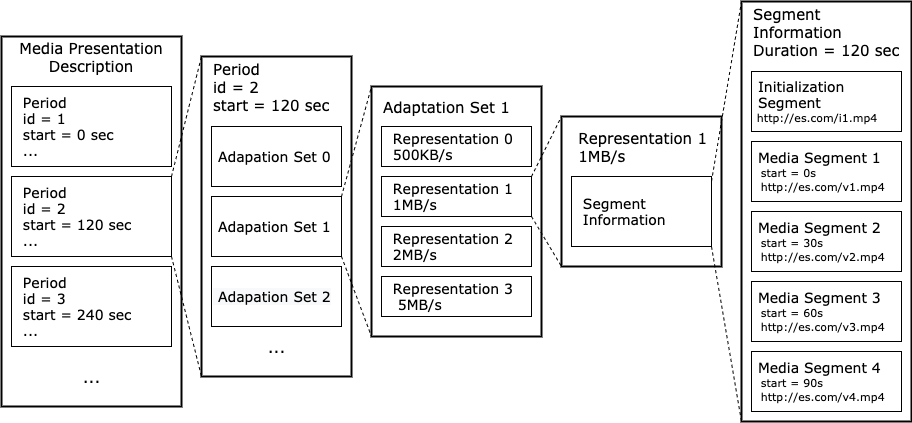
\includegraphics[width=\textwidth]{img/mpd.png}
  \caption{The MPD hierarchical data model. Source: MPEG \cite{ios1}}
  \label{fig:mpd}
\end{figure}

Each period consists of one or multiple \textbf{adaptation sets}. A collection of interchangeable 
encoded versions of one or more media content components is referred to as an adaptation set. For instance,
and adaptation set may contain the different bitrates of the video component of the same multimedia content
and another adaptation set may contain the different bitrates of the audio component of the same multimedia
content.

An adaptation set contains a set of \textbf{representations}, where a representation can be defined as an enconded
alternative of the same media component, representations are defined by parameters such as
bitrate, resolution, framerates, codec, sampling rate or other characteristics.

Each representation consists of one or multiple \textbf{segments}. A segment is a fragment of 
the multimedia content. Each segment is univocately identified by a \textit{URI}, the client 
sends \textit{HTTP} requests by using the \textit{URIs} to get the segments.


\subsection{Adaptation Algorithms}
\label{sec:adap}

In a video streaming service, factors such as the available bandwidth, delay or packet losses
can make the buffer to starve. Rebuffering and interruptions 
lead to bad Quality of Experience. To solve these problems, 
different adaptation algorithms have been proposed in the literature.

An adaptation algorithm is a technique used in a multimedia streaming service to adjust the video quality
in real-time according to different parameters. Some of the parameters are:

\begin{itemize}[noitemsep,topsep=0pt]
  \item \textbf{Client device}: The screen resolution, CPU capabilities, Buffer size, etc.
  \item \textbf{Network}: Type of access network (Mobile, Fixed), available bandwidth, etc.
\end{itemize}

The following subsections will explain different types of adaptation algorithms and the algorithms implemented
for this thesis in \textit{ns-3}.

\subsubsection{Bandwidth throughput based algorithms}

This group of algorithms uses bandwidth estimations to select
the most adequate multimedia representation. The main difference between algorithms of
this kind is the bandwidth estimation method and how the estimation influences
on the representation selection. 

\begin{figure}[h]
  \centering
  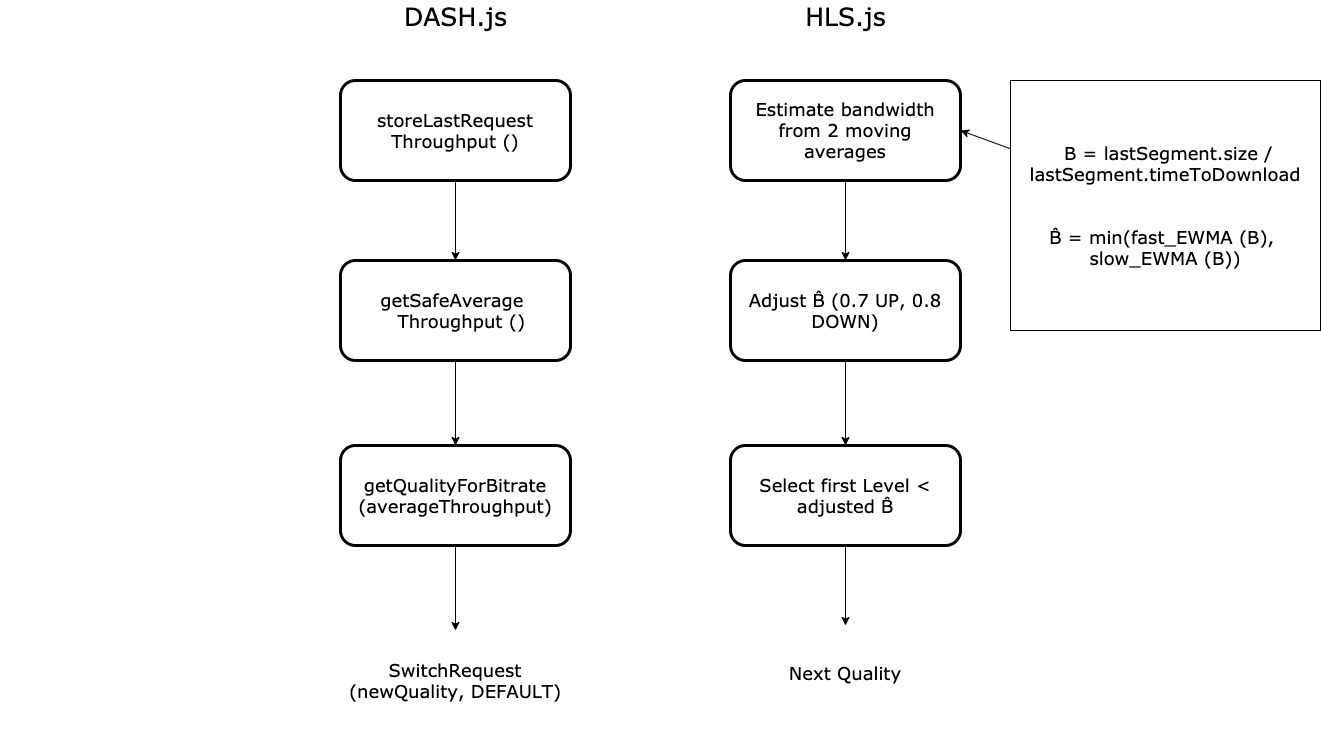
\includegraphics[width=\textwidth]{img/dashjs.png}
  \caption{Bandwidth based algorithms. Source: \cite{abr1}}
  \label{fig:throughput}
\end{figure}

\begin{itemize}
  \item \textbf{HLS.js} \cite{hls3}. The algorithm is called Bandwidth estimation. 
  
  The algorithm processes two EWMA (Exponentially Weighted Moving Averages) and chooses the minimum of the two 
  as the bandwidth estimation.

  \begin{equation}
    B_{N} = \frac{SegmentSize_{N}}{TimeToDownload_{N}} 
  \end{equation}


  \begin{gather}
    FastEWMA_{N} = B_{N} \times \alpha _{fast} +  FastEWMA_{N-1} \times (1 - \alpha _{fast}) \\
    SlowEWMA_{N} = B_{N} \times \alpha _{slow} +  SlowEWMA_{N-1} \times (1 - \alpha _{slow}) \\
    \hat{B} = min \,(FastEWMA_{N}, SlowEWMA_{N})
  \end{gather}

  Then the bandwidth estimation is multiplied by a factor to reduce oscilation. Finally it selects the 
  representation based on the adjusted bandwidth estimation. 



  \item \textbf{DASH.js} \cite{dash3}. Throughput Rule.
  
  This algorithm is basically the same as the Bandwidth estimation from HLS.js.
  It computes the average throughput, and uses an safety factor to avoid oscilations. And then chooses the quality
  based on the safe average and creates a new \textit{SwitchRequest}.

  
\end{itemize}

\subsubsection{Buffer based algorithms}

This group of algorithms uses buffer occupancy information to try to choose the highest level of bitrate
for the multimedia content.

\begin{itemize}
  \item \textbf{BOLA}. Buffer Occupancy based Lyapunov Algorithm.
  
  The BOLA adaptation algorithm uses the Lyapunov optimization \cite{bola1} to make decisions. This is an utility 
  theory and it is configurable with a tradeoff parameter to choose between rebuffering potential and bitrate
  maximization.
  
  \begin{figure}[h]
    \centering
    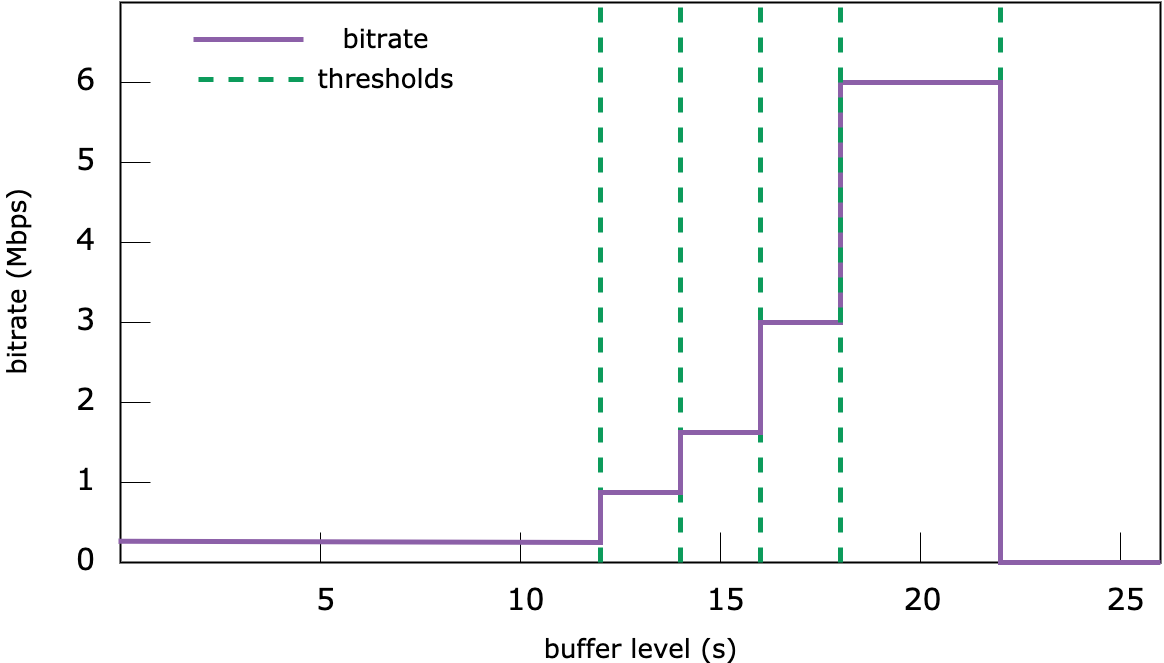
\includegraphics[width=0.75\textwidth]{img/BOLA.png}
    \caption{BOLA's bitrate choice as function of buffer level. Source: \cite{bola1}}
    \label{fig:bola}
  \end{figure}

  BOLA tries to maximize ${V_{n}+\gamma S_{n}}$.
  where: 
  \begin{itemize}
    \item[$\circ$] \textbf{${V_{n}}$} is the bitrate utility.
    \item[$\circ$] \textbf{${S_{n}}$} is the playback smoothness.
    \item[$\circ$] \textbf{${\gamma}$} is the tradeoff weight parameter for rebuffering potential or bitrate
    maximization.
  \end{itemize}
\end{itemize}


\subsubsection{Control theory based or hybrid algorithms}

This class of algorithms uses a combination of throughput estimation and buffer occupancy and tries to 
maximize the bitrate selection with decision-taking indicators calculated making use of control theory or
stochastic optimal control equations.

\subsection{QoS \& QoE Metrics}
\label{sec:qoemetrics}


The \textit{Quality of Service (QoS)} is defined by the \textit{ITU-T} in the document P.10/G.100
 \cite{itu2} as \textquotedbl The totality of characteristics of a telecommunications service that bear on its 
 ability to satisfy stated and implied needs of the user of the service\textquotedbl. And the \textit{Quality of 
Experience (QoE)} is defined as \textquotedbl The degree of delight or annoyance of the user of an application or service\textquotedbl.

The standard \textit{ISO/IEC 23009} defines a list of parameters for \textit{Quality of Service (QoS)} and
\textit{Quality of Experience (QoE)} for the adaptation algorithms to base on. There parameters 
are also used to evaluate the overall quality in the multimedia distribution service.

Some of the metrics defined in \cite{3gpp1} and \cite{ISO23009} are as follows:

\begin{itemize}
  \item \textbf{Average Throughput}: This is a \textit{QoE} metric that defines a list in which 
  the average throughput can be obtained that is observed in the client during a measuring period.
  \item \textbf{Initial Playout Delay}: This is a \textit{QoE} metric that represents the initial 
  delay in the reproduction of the media content.
  \item \textbf{Representation Switch Events}: This is a \textit{QoS} metric for measuring the 
  number of representation switch events of the multimedia content.
  \item \textbf{Buffer Level}: This is a \textit{QoS} metric that monitors the level of occupancy
  of the buffer during the reproduction of the multimedia content.
\end{itemize}


\section{LTE Fundamentals}
\label{sec:4g}

\textit{Long Term Evolution (LTE)} was first introduced in 2008 in the Release 8 of the \textit{3GPP}
specification \cite{lte1}. The objective of \textit{LTE} was to migrate the \textit{3GPP} systems
into a optimized system based on packet switching (all \textit{IP}), with greater bitrates, lower
latency y multiple radio access technologies support.

\subsection{History}
\label{sec:4gintro}

The first mobile phone call was made in 1973 \cite{mob1}. New generations of mobile networks 
are developed almost every decade. The first generation 1G launched years later, but
it was only capable of doing voice calls. In 1991, the second generation 2G \textit{(GSM)} of 
mobile networks was introduced. \textit{GSM} provided improved wireless capabilities and 
introduced by the first time multimedia content with \textit{Multimedia Message Service (MMS)}.
But it was the third generation 3G, launched in 2001, that enabled new internet-driven
services such as video conferencing and streaming. Later in 2009, the \textit{LTE} 4G standard
was commercially deployed. With theorical download bandwidth of almost 100Mbps made high-quality
streaming into reality. 5G technologies will provide an improvement in bandwidth even more and brings 
video streaming in \textit{UHD} and more.

The consumption of multimedia content on mobile networks is becoming increasingly relevant with 
the rise of bandwidth and ease of access. This section will provide a brief introduction to the 
basic concepts of mobile networks, their architecture and fundamentals.

\subsection{Architecture}
\label{sec:eps}

The design of the \textit{LTE} architecture was done from the ground up. The goal was to build a flat, all
\textit{IP} architecture using packet-switching, well structured (separation of control plane and user plane)
and with few elements.

\begin{figure}[h]
  \centering
  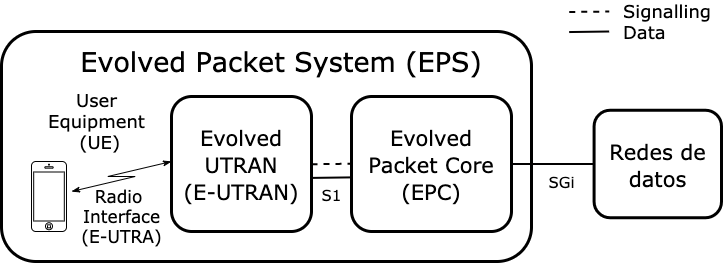
\includegraphics[width=0.8\textwidth]{img/eps.png}
  \caption{LTE Architecture}
  \label{fig:eps}
\end{figure}

The \textit{Evolved Packet System (EPS)} is constituted by the following elements:

\begin{itemize}
  \item \textbf{\textit{User Equipment (UE)}}: An \textit{UE} is any device used by an end user
  to communicate in a mobile network.
  \item \textbf{\textit{Evolved UMTS Terrestial Radio Access Network (E-UTRAN)}}: The only elements
  in the \textit{E-UTRAN} are the \textit{e-NodeB}. An \textit{\textbf{enhanced Node B (e-NodeB)}} works as a base station
  and a controller.
  \item \textbf{\textit{Evolved Packet Core (EPC)}}: The \textit{EPC} is made up of a network of gateways, 
  control servers, and databases linked by a \textit{IP} backbone. The main elements of the \textit{EPC}
  are:
  \begin{itemize}
    \item[$\circ$] \textit{\textbf{Mobility Management Entity (MME)}}: The \textit{MME} is 
    the main node for the control plane. It handles the signalling related to 
    mobility and security for \textit{E-UTRAN} access.
    \item[$\circ$] \textit{\textbf{Serving Gateway (SGW)}}: The \textit{SGW} is the gateway 
    used for communicating the access network \textit{E-UTRAN} and the \textit{PGW}.
    \item[$\circ$] \textit{\textbf{Packet Data Network Gateway (PGW)}}: The \textit{PGW} is the gateway
    for the traffic between the core network and external packet data networks. It also performs
    functions such as IP address allocation or packet filtering. 
    \item[$\circ$] \textit{\textbf{Home Subscriber Server (HSS)}}: The \textit{HSS} is a database 
    containing information about the \textit{EPC} network users.  It also provides support 
    functions in mobility management, call and session setup, user authentication and access authorization.
    \item[$\circ$] \textit{\textbf{Policy Charging and Rule Function (PCRF)}}: The \textit{PCRF} is used
    for \textit{QoS}, policy and charging management. 
  \end{itemize}
\end{itemize}

\begin{figure}[h]
  \centering
  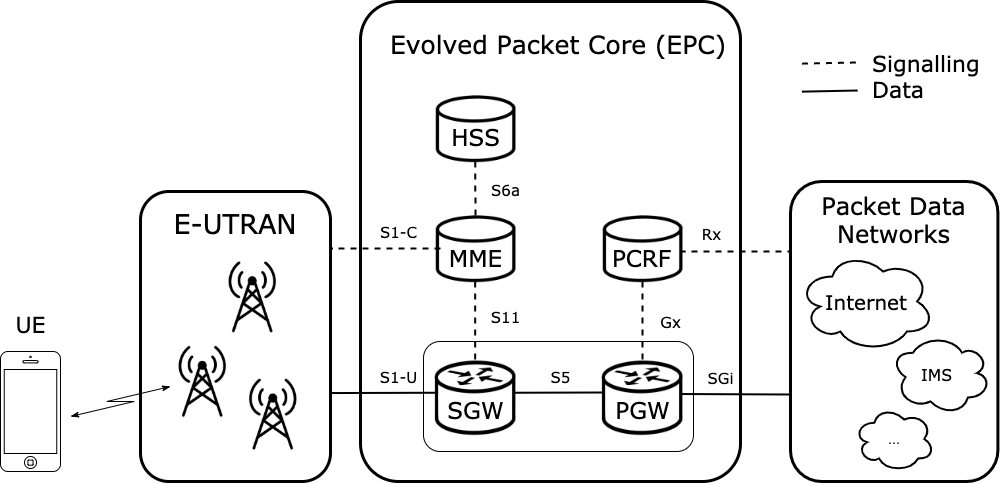
\includegraphics[width=0.8\textwidth]{img/epc.png}
  \caption{Evolved Packet Core (EPC) Architecture}
  \label{fig:epc}
\end{figure}

\subsection{Wireless Fundamentals}

Large-scale wireless networks, such as LTE, are fundamentally inefficient and prone to 
interference. Supporting mobility while also obtaining high levels of power efficiency, 
such as through directional antennas, can be really challenging. Base stations must be 
selectively installed but accommodate vast user populations in order to be cost-effective, 
resulting in a significant amount of self-interference. As a result, achieving high coverage, 
capacity, and dependability at low cost and used power is extremely difficult, if not impossible.

The following list highlights the main parameters affecting the received signal in a wireless system. 


\subsubsection{Propagation loss} 

The amount of transmitted power that actually reaches the receiver is the first visible 
difference between wired and wireless channels. The transmitted signal energy extends along 
a spherical wavefront if an isotropic antenna is utilized, hence the energy received at an 
antenna ${d}$ distant is inversely proportional to the sphere surface area, ${4\pi d^2}$.
However, in reality the propagation environment is not free space, we may also take into
account other factors such as reflections.

\subsubsection{Shadowing} 

Obstacles such as trees and buildings, as shown in Figure \ref{fig:pathloss}, may be situated between the 
transmitter and receiver, causing temporary signal degradation, whereas a temporary line-of-sight 
transmission path would result in abnormally high received power.

\begin{figure}[]
  \centering
  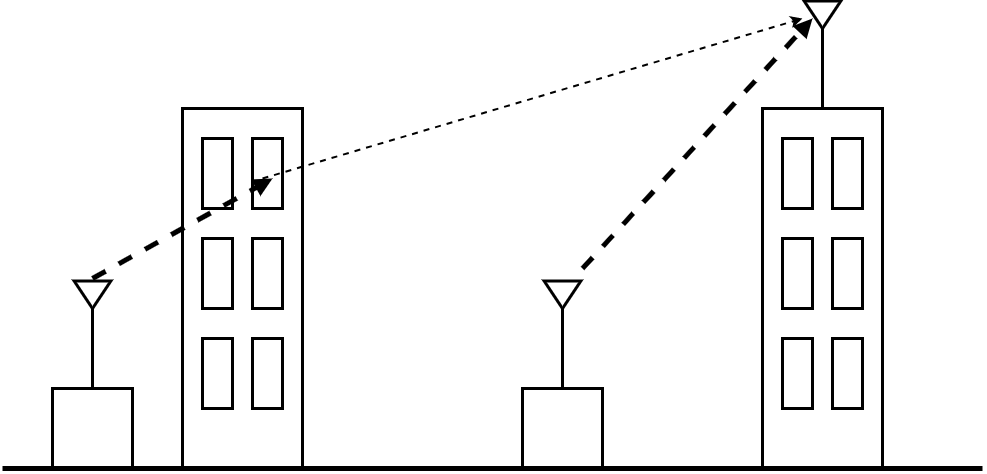
\includegraphics[width=0.77\textwidth]{img/pathloss.png}
  \caption{Shadowing effect. Source:\cite{lte2} }
  \label{fig:pathloss}
\end{figure}

\subsubsection{Fading loss} 

The fading effect is another aspect of wireless channels. Fading is generated by the receiving 
of multiple versions of the same signal (multipath), unlike path loss or shadowing, which are large-scale 
attenuation effects induced by distance or obstacles.

The reflections may arrive at very short intervals. For example, if there is local dispersion 
around the receiver, or they may arrive at relatively longer intervals, for instance, if the 
transmitter and receiver are on multiple pathways. Figure \ref{fig:fading} illustrates this.

\begin{figure}[]
  \centering
  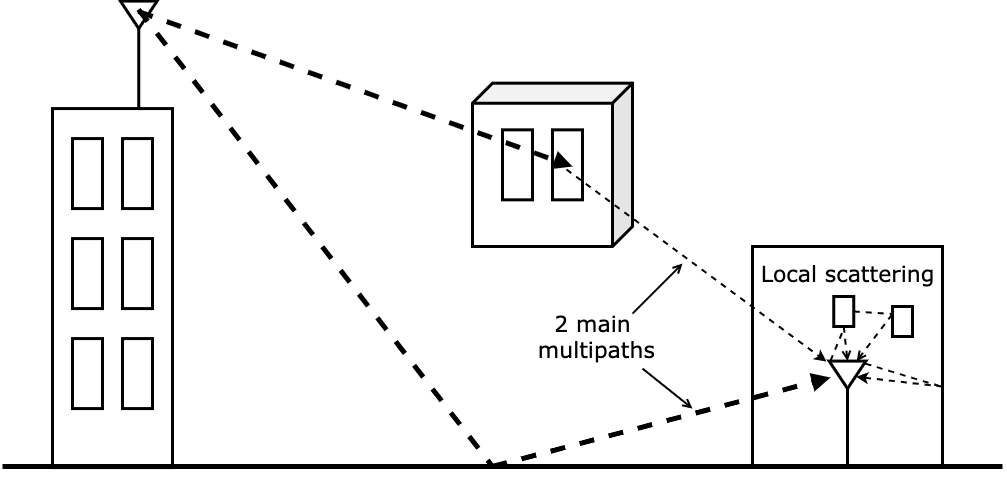
\includegraphics[width=0.77\textwidth]{img/fading.png}
  \caption{Fading loss effect. Source:\cite{lte2} }
  \label{fig:fading}
\end{figure}

\subsection{Antennas \& MIMO}

An antenna is a device that uses electromagnetic waves to transmit or receive information.
The transmitting antenna turns electrical currents into electromagnetic waves, 
and vice versa (receiving antenna).

\textit{Multiple Input, Multiple Output (MIMO)} is a technique for increasing the capacity 
of a radio link by employing multiple transmitting and receiving antennas to take advantage
of multipath propagation. MIMO has become a key component of wireless communication technologies 
such as LTE.

There are several implementations of MIMO in LTE:
\begin{itemize}[topsep=0pt]
  \item \textbf{\textit{Single antenna}}: Most simple wireless links employ this type of radio 
  transmission. One antenna transmits a single data stream, which is received by one or more 
  antennas. It is also know as SISO.
  \item \textbf{\textit{Transmit diversity}}: This type of LTE MIMO method makes use of several 
  antennas to transmit the same data stream.
  \item \textbf{\textit{Open loop spatial multiplexing}}: This type of MIMO involves delivering 
  two information streams through two or more antennas.
  \item \textbf{\textit{Close loop spatial multiplexing}}: Similar to the above but with a close 
  loop feedback.
  \item \textbf{\textit{Clesed loop with pre-coding}}: This type of MIMO transmits a single code word 
  over a single spatial layer.
  \item \textbf{\textit{Multi-User MIMO}}: Single-user SU-higher MIMO's per-user throughput is better 
  suited to more sophisticated user devices with more antennas, whereas MU-MIMO is more practical
  for low-complexity mobile phones with a small number of reception antennas.
  \item \textbf{\textit{Beam-forming \& MIMO}}: This is the most advanced MIMO mode. It allows
   the antenna to focus on a specific location.

\end{itemize}

\subsection{Physical Layer}



\subsubsection{OFDMA and SC-FDMA}
The cellular communication systems needs to have a strategy for multiple access. In LTE, the 
\textit{Orthogonal Frequency Division Multiple Access (OFDMA)} is used for downlink and the \textit{Single-
Carrier Frequency Division Multiple Access (SC-FDMA)} is used for uplink. Both are very similar, consisting
in allocating each subscriber some portion of the subcarriers for certain amount of time.

In the Figure \ref{fig:lterb}, a transmission structure of LTE is presented. The two dimentions of the 
plane are time and frequency. Two important concepts are defined as:

\begin{figure}[h]
  \centering
  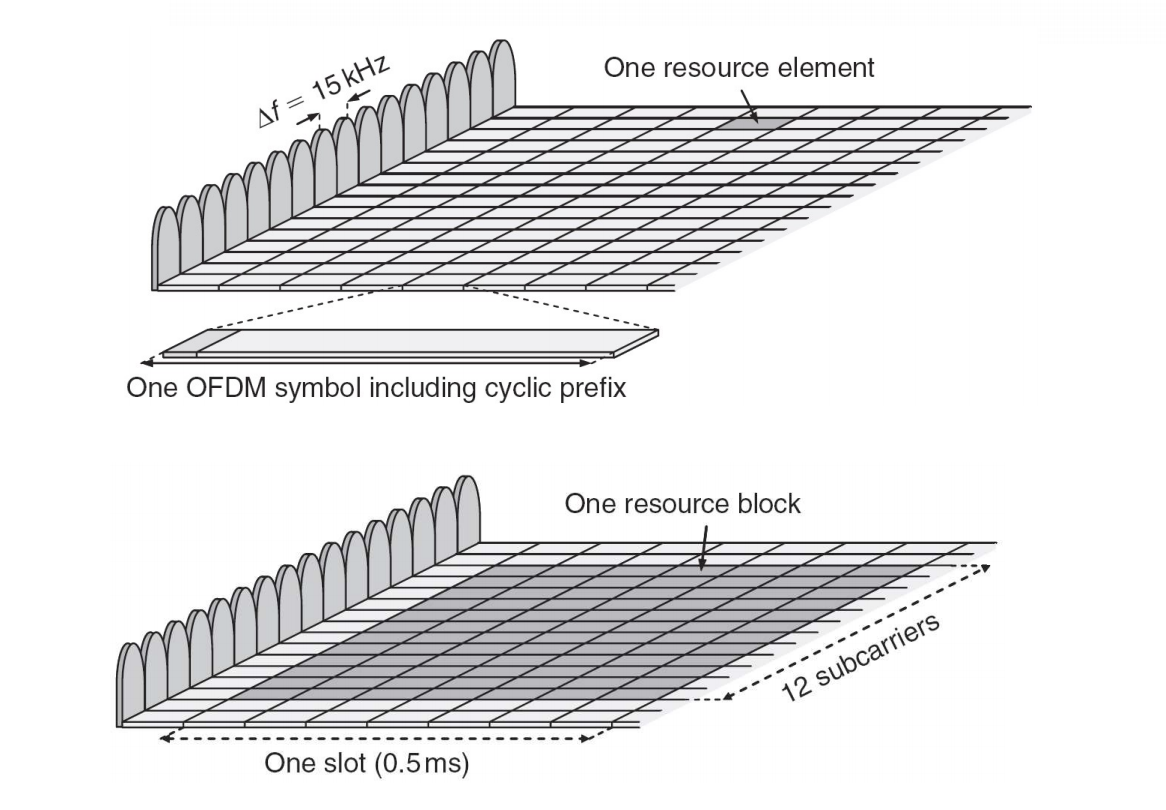
\includegraphics[width=0.95\textwidth]{img/lte_rb.png}
  \caption{LTE Time-Frequency Grid. Source:\cite{cmov1} }
  \label{fig:lterb}
\end{figure}

\begin{itemize}
  \item \textbf{\textit{Resource Element (RE)}}: A Resource Element is the basic element of resouce, it is
  defined as one subcarrier in a symbol period.
  \item \textbf{\textit{Resource Block (RB)}}: A Resource Block is composed by twelve subcarriers (180 kHz) in 
  a time interval of 0.5 ms (7 OFDM symbols).
\end{itemize}


Users are assigned resources in resource blocks across a subframe, i.e., 12 subcarriers over ${2\times7 = 14}$
OFDM symbols for a total of 168 Resource Elements. Because some of the 168 resource components are utilized 
for various layer 1 and layer 2 control messages, not all of them can be used for data.

The number of Resource Blocks available for each channel bandwidth is given by the Table \ref{table:rb}. 

\begin{table}[h]
  \centering
  \begin{tabular}{@{}lcccccc@{}}
  \toprule
  \textbf{Bandwidth}               & 1.4 MHz & 3 MHz & 5 MHz & 10 MHz & 15 MHz & 20 MHz \\ \midrule
  \textbf{Number of RBs available} & 6       & 15    & 25    & 50     & 75     & 100    \\ \bottomrule
  \end{tabular}
  \caption{Number of Resource Blocks against each channel bandwidth. Source: \cite{ofdma1}}
  \label{table:rb}
\end{table}

\subsubsection{AMC \& CQI}
AMC stands for Adaptive Modulation and Coding, is a terminology used in LTE
to describe how modulation and coding are matched to the radio link's conditions.

The eNB applies AMC by selecting the appropriate MCS based on quality estimations supplied 
by the UE mobile terminal via the \textit{Channel Quality Indication (CQI)} parameter.

\renewcommand{\arraystretch}{1}

\begin{table}[h]
  \centering

  \begin{tabular}{@{}cccc@{}}
  \toprule
  CQI Index & Modulation & Code Rate \textbackslash{}times 1024 & Efficiency \\ \midrule
  0         & \multicolumn{3}{c}{out of range}                               \\
  1         & QPSK       & 78                                   & 0.1523     \\
  2         & QPSK       & 120                                  & 0.2344     \\
  3         & QPSK       & 193                                  & 0.3770     \\
  4         & QPSK       & 308                                  & 0.6016     \\
  5         & QPSK       & 449                                  & 0.8770     \\
  6         & QPSK       & 602                                  & 1.1758     \\
  7         & 16QAM      & 378                                  & 1.4766     \\
  8         & 16QAM      & 490                                  & 1.9141     \\
  9         & 16QAM      & 616                                  & 2.4063     \\
  10        & 64QAM      & 466                                  & 2.7305     \\
  11        & 64QAM      & 567                                  & 3.3223     \\
  12        & 64QAM      & 666                                  & 3.9023     \\
  13        & 64QAM      & 772                                  & 4.5234     \\
  14        & 64QAM      & 873                                  & 5.1152     \\
  15        & 64QAM      & 948                                  & 5.5547     \\ \bottomrule
  \end{tabular}
  \caption{4-Bit CQI Table}
\end{table}
MCS

\subsubsection{EARFCN}
The \textit{E-UTRA Absolute Radio Frequency Channel Number (EARFCN)} is a number between 0-65535 used
for desginating uplink and downlink carrier frequencies.

\begin{align}
  F_{downlink} = FDL_{Low} + 0.1 (NDL - NDL_{Offset})\\
  F_{uplink} = FUL_{Low} + 0.1 (NUL - NUL_{Offset})
\end{align}

Where ${NDL}$ is the downlink EARFCN, ${NUL}$ is the uplink EARFCN.

\subsubsection{Souding Reference Signal}
\textit{Souding Reference Signal (SRS)} are wideband reference signals used by the eNode-B to determine uplink channel quality information 
in order to allocate uplink resources. There are three types of SRS transmissions, single SRS, periodic SRS and aperiodic SRS.


\subsection{Medium Access Control Layer}
The \textit{Medium Access Controll (MAC)} layer essentially provides the higher layer with radio
resource allocation and data transfer services and connects the RLC layer and the PHY layer. 
The MAC layer executes procedures such as logical channel priority, power headroom reporting,
UL grant and DL assignment, and so on as part of the radio resource allocation service.
The MAC layer performs functions like scheduling requests, buffer status reporting, random access, 
and HARQ as part of the data transmission service.

\subsection{Radio Link Control Layer}
The RLC layers's key functions include data unit segmentation and concatenation, 
error correction via the ARQ protocol, and packet delivery 
in sequence to higher levels. It has three modes of operation:

\begin{itemize}[noitemsep,topsep=0pt]
  \item \textbf{Transparent Mode (TM)} is the most basic mode, with no RLC header, 
  data segmentation, or concatenation, and is used for specialized applications 
  like random access.
  \item \textbf{Unacknowledged Mode (UM)} The UM mode detects packet loss and allows 
  for packet reordering and reassembly, 
  but does not require the missing protocol data units to be retransmitted (PDUs).
  \item \textbf{Acknowledged Mode (AM)} is set up to request retransmission of missing 
  PDUs in addition to the UM mode's features.
\end{itemize}

\subsection{Packet Data Convergence Protocol Layer}


The PDCP layer's main features are IP packet header compression and decompression 
based on the \textit{RObust Header Compression (ROHC)} protocol, data and signaling ciphering, 
and signaling integrity protection. Per bearer, there is only one PDCP entity at the 
eNode-B and the UE.








